% \usetikzlibrary{calc,positioning,shapes.geometric}
\resizebox{\columnwidth}{!}{%
\begin{tikzpicture}[font=\sffamily\Huge     ]

% ============================================================
% LEFT PART: 4 target diagrams
% ============================================================
\def\targetcircle{
  \fill[white] (0,0) circle (1);
  \fill[red!85!black] (0,0) circle (0.72);
  \fill[white] (0,0) circle (0.46);
  \fill[red!85!black] (0,0) circle (0.14);
  \draw[black,thin] (0,0) circle (1);
}

% --- Target 1: Low accuracy, Low precision ---
\begin{scope}[shift={(0,3.4)}]
  \targetcircle
  \foreach \p in {(-0.55,0.25),(0.68,0.42),(-0.28,-0.72),(0.5,-0.55),
                  (-0.82,-0.15),(0.18,0.82),(0.85,-0.22),(-0.15,0.05)}
    \fill \p circle (2.2pt);
  \node[anchor=west,align=left,font=\sffamily\small] at (0.75,1.15) {Low accuracy\\Low precision};
\end{scope}

% --- Target 2: Low accuracy, High precision ---
\begin{scope}[shift={(2.6,3.4)}]
  \targetcircle
  \foreach \p in {(-0.55,0.55),(-0.62,0.62),(-0.5,0.68),(-0.68,0.5),
                  (-0.58,0.48),(-0.45,0.6),(-0.6,0.4)}
    \fill \p circle (2.2pt);
  \node[anchor=west,align=left,font=\sffamily\small] at (0.75,1.15) {Low accuracy\\High precision};
\end{scope}

% --- Target 3: High accuracy, Low precision ---
\begin{scope}[shift={(0,0.8)}]
  \targetcircle
  \foreach \p in {(-0.3,0.2),(0.25,0.3),(-0.22,-0.25),(0.3,-0.15),
                  (0.05,0.35),(-0.35,-0.05),(0.1,-0.32)}
    \fill \p circle (2.2pt);
  \node[anchor=west,align=left,font=\sffamily\small] at (0.75,1.15) {High accuracy\\Low precision};
\end{scope}

% --- Target 4: High accuracy, High precision ---
\begin{scope}[shift={(2.6,0.8)}]
  \targetcircle
  \foreach \p in {(0,0),(0.06,0.05),(-0.05,0.04),(0.04,-0.06),
                  (-0.04,-0.04),(0.02,0.08),(-0.06,-0.02)}
    \fill \p circle (2.2pt);
  \node[anchor=west,align=left,font=\sffamily\small] at (0.75,1.15) {High accuracy\\High precision};
\end{scope}

% ============================================================
% MIDDLE PART: confusion matrix
% ============================================================
\begin{scope}[shift={(8,0)}]

  % cell dimensions
  \def\w{3}
  \def\h{2}

  % --- colored outline rectangles (drawn back to front) ---
  % Accuracy - blue - whole square
  \draw[line width=1.6pt, cyan!70, rounded corners=14pt]
    (-0.55,-0.55) rectangle (2*\w+0.55, 2*\h+0.55);

  % Recall - pink - top row
  \draw[line width=1.6pt, purple!80, rounded corners=10pt]
    (-0.35,\h+0.2) rectangle (2*\w+0.35, 2*\h+0.35);

  % Specificity - orange - bottom row
  \draw[line width=1.6pt, orange!90, rounded corners=10pt]
    (-0.35,-0.35) rectangle (2*\w+0.35, \h-0.2);

  % Precision - green - left column
  \draw[line width=1.6pt, teal!80, rounded corners=8pt]
    (-0.15,-0.15) rectangle (\w+0.15, 2*\h+0.15);

  % --- grid divider lines (dotted) ---
  \draw[dotted, gray] (0,\h) -- (2*\w,\h);
  \draw[dotted, gray] (\w,0) -- (\w,2*\h);

  % --- cell text ---
  \node[align=center] at (0.5*\w, 1.6*\h) {True\\Positive};
  \node[align=center] at (1.5*\w, 1.6*\h) {False\\Negative};
  \node[align=center] at (0.5*\w, 0.4*\h) {False\\Positive};
  \node[align=center] at (1.5*\w, 0.4*\h) {True\\Negative};

  % --- column headers ---
  \node[font=\sffamily\Large] at (0.5*\w, 2*\h+1.0) {Species$_k$};
  \node[font=\sffamily\Large] at (1.5*\w, 2*\h+1.0) {Other sp.};
  \node[font=\sffamily\Large] at (\w, 2*\h+1.7) {Predicted};

  % --- row headers ---
  \node[font=\sffamily\Large, rotate=90] at (-1.6, 1.5*\h) {Species$_k$};
  \node[font=\sffamily\Large, rotate=90] at (-1.6, 0.5*\h) {Other sp.};
  \node[font=\sffamily\Large, rotate=90] at (-2.35, \h) {Observed};

\end{scope}

% ============================================================
% RIGHT PART: legend with formulas
% ============================================================
\begin{scope}[shift={(15.2,0)}]

  \def\rowsep{1.35}

  % Accuracy - row 4 (top)
  \node[fill=cyan!70, minimum width=0.9cm, minimum height=0.9cm] (sq1) at (0,3*\rowsep) {};
  \node[anchor=west, font=\sffamily\Large] at (0.7,3*\rowsep) {Accuracy};
  \node[anchor=west, font=\sffamily\large] at (3.1,3*\rowsep) {=};
  \node[anchor=west] at (3.6,3*\rowsep) {$\dfrac{\text{TP}+\text{TN}}{\text{TP}+\text{TN}+\text{FP}+\text{FN}}$};

  % Specificity - row 3
  \node[fill=orange!90, minimum width=0.9cm, minimum height=0.9cm] (sq2) at (0,2*\rowsep) {};
  \node[anchor=west, font=\sffamily\Large] at (0.7,2*\rowsep) {Specificity};
  \node[anchor=west, font=\sffamily\large] at (3.1,2*\rowsep) {=};
  \node[anchor=west] at (3.6,2*\rowsep) {$\dfrac{\text{TN}}{\text{TN}+\text{FP}}$};

  % Precision - row 2
  \node[fill=teal!80, minimum width=0.9cm, minimum height=0.9cm] (sq3) at (0,1*\rowsep) {};
  \node[anchor=west, font=\sffamily\Large] at (0.7,1*\rowsep) {Precision};
  \node[anchor=west, font=\sffamily\large] at (3.1,1*\rowsep) {=};
  \node[anchor=west] at (3.6,1*\rowsep) {$\dfrac{\text{TP}}{\text{TP}+\text{FP}}$};

  % Recall - row 1 (bottom)
  \node[fill=purple!80, minimum width=0.9cm, minimum height=0.9cm] (sq4) at (0,0) {};
  \node[anchor=west, font=\sffamily\Large] at (0.7,0) {Recall};
  \node[anchor=west, font=\sffamily\large] at (3.1,0) {=};
  \node[anchor=west] at (3.6,0) {$\dfrac{\text{TP}}{\text{TP}+\text{FN}}$};

\end{scope}

\end{tikzpicture}
}